\documentclass[10pt]{beamer}

% ------------------------------------------------------------------------
% Carga del preámbulo personalizado
% (Asegúrate de contar con preamble.tex en la misma carpeta,
%  donde defines temas, colores, macros como \myfront, etc.)
% ------------------------------------------------------------------------
\usetheme[progressbar=frametitle]{metropolis}
\usepackage{appendixnumberbeamer}
\usepackage{fancyvrb}
\usepackage{booktabs}
\usepackage[scale=2]{ccicons}
\usepackage{pgfplots}
\usepgfplotslibrary{dateplot}
\usepackage{type1cm}
\usepackage{lettrine}
\usepackage{ragged2e}
\usepackage{xspace}
\newcommand{\themename}{\textbf{\textsc{metropolis}}\xspace}
\usepackage{graphicx} % Allows including images
\usepackage{booktabs} % Allows the use of \toprule, \midrule and \bottomrule in tables
\usepackage[utf8]{inputenc} %solucion del problema de los acentos.
\usepackage{xcolor}
\definecolor{LightGray}{gray}{0.9}

\usepackage{minted}
\usemintedstyle{tango}
\newcommand{\mypyfile}[1]{\inputminted[linenos=true, fontsize=\footnotesize, frame=lines, framesep=5\fboxrule,framerule=1pt]{python}{#1}}

\setminted[python]{breaklines,frame=lines,framesep=2mm,baselinestretch=1.2,bgcolor=LightGray,linenos, fontsize=\footnotesize} % obeytabs=true, tabsize=2, showtabs=true}

%%%%%%%%%%%%%%%%%%%%%%%%%%%%%%%%%%%%%%%%%%%%%%%%%%%%%%%%%%%%%%%%%%%%%%%%%%%%%%%%%%%%%%
\setbeamercolor{progress bar}{fg=blue!50!black,bg=white!50!black}
\setbeamercolor{title separator}{fg=red!50!black,bg=white!50!black}
\setbeamercolor{frametitle}{fg=white!80!black,bg=red!50!black}
\title[PCFI161]{Programaci\'on para F\'isica y Astronom\'ia}
\subtitle{Departamento de Física.}

\newcommand{\myfront}{
\author[PCFI161]{Corodinadora: C Loyola \\ Profesoras/es C Loyola / C Femenías / Y Navarrete / C Ruiz}
\institute[UNAB]{Universidad Andrés Bello}
\date{Primer Semestre 2025}
}

\titlegraphic{%
  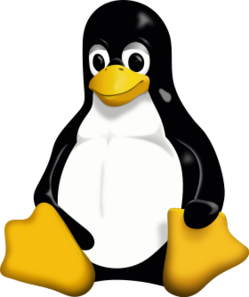
\includegraphics[width=.08\textwidth]{logo-tux.png}\hfill
  
\includegraphics[width=.3\textwidth]{logo-unab.png}\hfill
  
\includegraphics[width=.08\textwidth]{logo-python.png}
}

\makeatletter
\setbeamertemplate{title page}{
  \begin{minipage}[b][\paperheight]{\textwidth}
    \vfill%
    \ifx\inserttitle\@empty\else\usebeamertemplate*{title}\fi
    \ifx\insertsubtitle\@empty\else\usebeamertemplate*{subtitle}\fi
    \usebeamertemplate*{title separator}
    \ifx\beamer@shortauthor\@empty\else\usebeamertemplate*{author}\fi
    \ifx\insertdate\@empty\else\usebeamertemplate*{date}\fi
    \ifx\insertinstitute\@empty\else\usebeamertemplate*{institute}\fi
    \vfill
    \ifx\inserttitlegraphic\@empty\else\inserttitlegraphic\fi
    \vspace*{1cm}
  \end{minipage}
}
\makeatother


\makeatletter
\setlength{\metropolis@titleseparator@linewidth}{2pt}
\setlength{\metropolis@progressonsectionpage@linewidth}{2pt}
\setlength{\metropolis@progressinheadfoot@linewidth}{2pt}
\makeatother


\begin{document}

% ------------------------------------------------------------------------
% Portada personalizada. Por ejemplo, usando \myfront si lo tienes en el preámbulo.
% ------------------------------------------------------------------------
\myfront{}

% ------------------------------------------------------------------------
% SLIDE 1: Título de la segunda sesión
% ------------------------------------------------------------------------
\begin{frame}
  \titlepage
  % Puedes ajustar el título/subtítulo para esta sesión específica
  % por ejemplo: \title{Sesión 2 - Semana 1: Ejercicios Iniciales en Colab}
\end{frame}

% ------------------------------------------------------------------------
% SLIDE 2: Índice / Tabla de contenidos
% ------------------------------------------------------------------------
\begin{frame}
  \frametitle{Resumen - Sesión 2 (Semana 1)}
  \tableofcontents
\end{frame}

% ------------------------------------------------------------------------
% Configuración de bloques (en caso de usar metrópolis u otro tema)
% ------------------------------------------------------------------------
\metroset{block=fill}

% ----------------------------------------------------------------------------------------
% SECCIÓN 1: Recapitulación de la Sesión 1
% ----------------------------------------------------------------------------------------
\section{Recapitulación Sesión 1}

% ------------------------------------------------------------------------
% Slide 3: Repaso Rápido
% ------------------------------------------------------------------------
\begin{frame}{Repaso de la Clase Anterior}
  \begin{itemize}
    \item Contexto general del curso y relevancia de la programación en Física/Astronomía.
    \item Familiarización inicial con Google Colab:
      \begin{itemize}
        \item Creación de notebooks.
        \item Ejecución de código básico.
      \end{itemize}
    \item Introducción a los tipos de datos y operaciones simples (asignaciones, suma, resta, etc.).
    \item Primeros ejemplos de entrada y salida (\texttt{input()}, \texttt{print()}).
  \end{itemize}
\end{frame}

% ------------------------------------------------------------------------
% Slide 4: Objetivos de Esta Sesión
% ------------------------------------------------------------------------
\begin{frame}{Objetivos de la Sesión 2}
  \begin{itemize}
    \item \textbf{Practicar} asignaciones simples y operaciones aritméticas en Colab.
    \item \textbf{Explorar} más ejemplos de entrada/salida y la ejecución inmediata de código.
    \item \textbf{Fomentar} la colaboración e intercambio de estrategias entre estudiantes.
    \item \textbf{Resolver} ejercicios que integren los conceptos vistos en la sesión anterior.
  \end{itemize}
\end{frame}

% ----------------------------------------------------------------------------------------
% SECCIÓN 2: Ajustes y Entorno en Colab
% ----------------------------------------------------------------------------------------
\section{Ajustes y Entorno en Colab}

% ------------------------------------------------------------------------
% Slide 5: Organización de Archivos
% ------------------------------------------------------------------------
\begin{frame}{Organización de Archivos y Notebooks}
  \begin{itemize}
    \item Es recomendable mantener una carpeta específica para la asignatura en Google Drive.
    \item Crearemos un notebook llamado \texttt{Sesion2\_Semana1.ipynb} para guardar nuestro trabajo.
    \item \textbf{Tip:} Usa nombres descriptivos para notebooks y subcarpetas (e.g., \emph{ejercicios}, \emph{notas}, \emph{pruebas}).
  \end{itemize}
\end{frame}

% ------------------------------------------------------------------------
% Slide 6: Ejecución Inmediata de Código
% ------------------------------------------------------------------------
\begin{frame}[fragile]{Ejecución Inmediata de Código en Colab}
  \begin{itemize}
    \item Cada celda de un notebook se ejecuta de forma independiente.
    \item Es posible realizar pruebas rápidas sin afectar las demás celdas.
    \item \textbf{Ejemplo de celda interactiva}:
    \begin{minted}[
      frame=lines,
      framesep=2mm,
      baselinestretch=1.2,
      bgcolor=LightGray,
      fontsize=\footnotesize
    ]{python}
# Celda 1
x = 10
print(x)
    \end{minted}

    \begin{minted}[
      frame=lines,
      framesep=2mm,
      baselinestretch=1.2,
      bgcolor=LightGray,
      fontsize=\footnotesize
    ]{python}
# Celda 2
x = x + 5
print(x)  # Mostrará 15
    \end{minted}
  \end{itemize}
\end{frame}

% ----------------------------------------------------------------------------------------
% SECCIÓN 3: Ejercicios de Asignaciones y Operaciones
% ----------------------------------------------------------------------------------------
\section{Ejercicios de Asignaciones y Operaciones}

% ------------------------------------------------------------------------
% Slide 7: Ejercicio 1 - Conversión de Unidades
% ------------------------------------------------------------------------
\begin{frame}{Ejercicio 1: Conversión de Unidades}
  \begin{block}{Enunciado}
    \begin{itemize}
      \item Pide al usuario que introduzca una longitud en \textbf{metros}.
      \item Convierte ese valor a centímetros, milímetros y kilómetros.
      \item Imprime los resultados.
    \end{itemize}
  \end{block}
  \textbf{Objetivo:} Practicar asignaciones simples, multiplicaciones y/o divisiones.
\end{frame}

% ------------------------------------------------------------------------
% Slide 8: Ejercicio 2 - Suma de Dos Variables
% ------------------------------------------------------------------------
\begin{frame}{Ejercicio 2: Suma de Dos Variables}
  \begin{block}{Enunciado}
    \begin{itemize}
      \item Pide al usuario dos números (pueden ser enteros o decimales).
      \item Asigna cada número a una variable distinta (\texttt{a, b}).
      \item Realiza la suma y muestra el resultado.
    \end{itemize}
  \end{block}
  \textbf{Extensión:} Imprime también la resta, el producto y el cociente.
\end{frame}

% ------------------------------------------------------------------------
% Slide 9: Ejercicio 3 - Promedio de Tres Notas
% ------------------------------------------------------------------------
\begin{frame}{Ejercicio 3: Promedio de Tres Notas}
  \begin{block}{Enunciado}
    \begin{itemize}
      \item Solicita tres notas (numeros en \([1.0 - 7.0]\) típicamente).
      \item Calcula el promedio aritmético.
      \item Muestra el resultado con un mensaje apropiado.
    \end{itemize}
  \end{block}
  \textbf{Discusión:}
  \begin{itemize}
    \item ¿Qué pasa si ingresan valores fuera del rango?
    \item El tipo de dato a usar: \texttt{float}.
  \end{itemize}
\end{frame}

% ----------------------------------------------------------------------------------------
% SECCIÓN 4: Resolución Colaborativa
% ----------------------------------------------------------------------------------------
\section{Resolución Colaborativa}

% ------------------------------------------------------------------------
% Slide 10: Grupos de Trabajo
% ------------------------------------------------------------------------
\begin{frame}{Trabajo en Grupos}
  \begin{itemize}
    \item Dividir la clase en \textbf{equipos de 2-3 integrantes}.
    \item Cada equipo crea o comparte un notebook en Colab con sus compañeros.
    \item Se recomienda comentar el código para anotar:
      \begin{itemize}
        \item Qué hace cada línea.
        \item Si surge algún error, cómo se corrigió.
      \end{itemize}
    \item Comparar sus resultados y conclusiones.
  \end{itemize}
\end{frame}

% ------------------------------------------------------------------------
% Slide 11: Puesta en Común
% ------------------------------------------------------------------------
\begin{frame}{Puesta en Común de Dudas y Experiencias}
  \begin{itemize}
    \item Cada equipo expondrá brevemente:
      \begin{itemize}
        \item ¿Qué ejercicio les costó más y por qué?
        \item ¿Cómo resolvieron los problemas encontrados?
        \item ¿Algún atajo o truco que consideren útil?
      \end{itemize}
    \item Se fomenta la retroalimentación colectiva.
    \item \textbf{Tip:} Documentar buenas prácticas que surjan de la discusión.
  \end{itemize}
\end{frame}

% ------------------------------------------------------------------------
% Slide 12: Ejemplo de Solución (Conversión de Unidades)
% ------------------------------------------------------------------------
\begin{frame}[fragile]{Ejemplo de Solución: Conversión de Unidades}
\begin{minted}[
frame=lines,
framesep=2mm,
baselinestretch=1.1,
bgcolor=LightGray,
fontsize=\footnotesize
]{python}
long_m = float(input("Introduce una longitud en metros: "))
cm = long_m * 100
mm = long_m * 1000
km = long_m / 1000

print(f'En centímetros: {cm} cm')
print(f'En milímetros : {mm} mm')
print(f'En kilómetros : {km} km')
\end{minted}
\end{frame}

% ------------------------------------------------------------------------
% Slide 13: Ejemplo de Solución (Suma de Dos Variables)
% ------------------------------------------------------------------------
\begin{frame}[fragile]{Ejemplo de Solución: Suma de Dos Variables}
\begin{minted}[
frame=lines,
framesep=2mm,
baselinestretch=1.1,
bgcolor=LightGray,
fontsize=\footnotesize
]{python}
a_str = input("Ingresa el primer número: ")
b_str = input("Ingresa el segundo número: ")

a = float(a_str)
b = float(b_str)

suma = a + b
resta = a - b
producto = a * b
cociente = a / b  # Cuidar la división por cero

print(f'Suma = {suma}')
print(f'Resta = {resta}')
print(f'Producto = {producto}')
print(f'Cociente = {cociente}')
\end{minted}
\end{frame}

% ------------------------------------------------------------------------
% Slide 14: Ejemplo de Solución (Promedio de Tres Notas)
% ------------------------------------------------------------------------
\begin{frame}[fragile]{Ejemplo de Solución: Promedio de Tres Notas}
\begin{minted}[
frame=lines,
framesep=2mm,
baselinestretch=1.1,
bgcolor=LightGray,
fontsize=\footnotesize
]{python}
n1 = float(input("Nota 1: "))
n2 = float(input("Nota 2: "))
n3 = float(input("Nota 3: "))

promedio = (n1 + n2 + n3) / 3
print(f'El promedio de las tres notas es: {promedio}')
\end{minted}
\textbf{Discusión:} Manejo de rangos y validaciones (opcional).
\end{frame}

% ------------------------------------------------------------------------
% Slide 15: Pequeña Discusión sobre Errores
% ------------------------------------------------------------------------
\begin{frame}{Errores Frecuentes en Python}
  \begin{itemize}
    \item \textbf{ValueError}: ocurre al convertir strings inválidos en \texttt{float} o \texttt{int}.
    \item \textbf{ZeroDivisionError}: cuando \texttt{b = 0} y se hace \texttt{a/b}.
    \item \textbf{NameError}: uso de variables no definidas o mal escritas.
  \end{itemize}
  \textbf{Tip:} Leer atentamente el mensaje de error para identificar la causa y línea afectada.
\end{frame}

% ----------------------------------------------------------------------------------------
% SECCIÓN 5: Actividad Adicional y Retroalimentación
% ----------------------------------------------------------------------------------------
\section{Actividades Prácticas}

% ------------------------------------------------------------------------
% Slide 16: Actividad Extra - Escalas Físicas
% ------------------------------------------------------------------------
\begin{frame}{Actividad: Escalas Físicas}
  El objetivo de esta actividad es de práctica en casa, la idea es que pueda prepararse para la Tarea en clase de la próxima semana que se realizará en la sesión 2.
  \begin{block}{Enunciado}
    \begin{itemize}
      \item Pide la temperatura en \(^\circ C\) y conviértela a \(^\circ F\) y K.
      \item Pide la masa en kg y conviértela a libras.
      \item Muestra un pequeño resumen en pantalla con los resultados.
    \end{itemize}
  \end{block}
  \textbf{Objetivo:} Reforzar uso de variables, operaciones aritméticas y \texttt{print}.
\end{frame}

% ------------------------------------------------------------------------
% Slide 17: Mini-Reto - Operaciones con Complejos
% ------------------------------------------------------------------------
\begin{frame}{Mini-Reto: Números Complejos (Opcional)}
  \begin{itemize}
    \item Python maneja complejos con la letra \texttt{j} (\emph{ej}: \texttt{3+2j}).
    \item Investiga cómo sumar, restar y multiplicar números complejos.
    \item \textbf{Ejemplo}:
      \[
        z1 = 3 + 4j, \quad z2 = 2 - 1j
      \]
      \[
        z3 = z1 * z2
      \]
      \(\dots\) Imprime \(\operatorname{Re}(z3)\) y \(\operatorname{Im}(z3)\).
    \item \textbf{Tip}: Usa \texttt{z.real} y \texttt{z.imag} para acceder a sus partes real e imaginaria.
  \end{itemize}
\end{frame}

% ------------------------------------------------------------------------
% Slide 18: Momento de Discusión
% ------------------------------------------------------------------------
\begin{frame}{Discusión Grupales y Dudas}
  \begin{itemize}
    \item ¿Qué soluciones o trucos surgieron durante la actividad extra?
    \item ¿Se presentaron nuevas dudas o errores inesperados?
    \item ¿Qué parte de Python se está volviendo más clara y qué sigue siendo confuso?
  \end{itemize}
  \begin{block}{IMPORTANTE!!!}
    Los resultados de su trabajo en clases deben ser entregados mediante la plataforma CANVAS.
  \end{block}
\end{frame}

% ------------------------------------------------------------------------
% Slide 19: Retroalimentación y Comentarios
% ------------------------------------------------------------------------
\begin{frame}{Retroalimentación}
  \begin{itemize}
    \item Comparte tu experiencia de aprendizaje con tus compañeros.
    \item \textbf{Ventajas} de Colab: ejecución inmediata, trabajo colaborativo, fácil despliegue de resultados.
    \item \textbf{Desafíos} detectados: conexión a internet, diferencia de versiones, etc.
  \end{itemize}
\end{frame}

% ----------------------------------------------------------------------------------------
% SECCIÓN 6: Conclusiones y Próximos Pasos
% ----------------------------------------------------------------------------------------
\section{Conclusiones}

% ------------------------------------------------------------------------
% Slide 20: Resumen de la Sesión 2
% ------------------------------------------------------------------------
\begin{frame}{Resumen de la Sesión 2}
  \begin{itemize}
    \item Reforzamos las operaciones básicas y la asignación de variables.
    \item Practicamos \textbf{entrada/salida} con varios ejemplos.
    \item Exploramos la \textit{ejecución inmediata} de celdas en Colab y la importancia del orden.
    \item Fomentamos la resolución colaborativa para intercambiar estrategias.
  \end{itemize}
\end{frame}

% ------------------------------------------------------------------------
% Slide 21: Enfoque para la Próxima Sesión
% ------------------------------------------------------------------------
\begin{frame}{Próximos Pasos}
  \begin{itemize}
    \item \textbf{Sesión 3 (Semana 2)}: Introducción a estructuras de control (\texttt{if}, \texttt{while}).
    \item \textbf{Explotaremos} ejemplos físicos básicos (análisis de condiciones, pequeños bucles, etc.).
    \item \textbf{Revisión previa}: Asegúrate de dominar los \textbf{tipos de datos} y la conversión de \texttt{input()} a \texttt{float}.
  \end{itemize}
\end{frame}

% ------------------------------------------------------------------------
% Slide 22: Referencias y Recursos
% ------------------------------------------------------------------------
\begin{frame}{Recursos Recomendados}
  \begin{itemize}
    \item \textbf{Documentación Python:} \href{https://docs.python.org/3/}{docs.python.org/3}
    \item \textbf{Tutoriales en línea:} W3Schools, Real Python.
    \item \textbf{Comunidades:} Stack Overflow, Reddit \texttt{/r/learnpython}.
    \item \textbf{GitHub:} Busca \emph{“intro to python for physics”} para ejemplos.
  \end{itemize}
\end{frame}

% ------------------------------------------------------------------------
% Slide 23: Comentarios Finales
% ------------------------------------------------------------------------
\begin{frame}{Comentarios Finales}
  \begin{itemize}
    \item \textbf{Practicar} es fundamental: domina bien asignaciones y operaciones antes de pasar a estructuras más complejas.
    \item \textbf{Comparte} dudas en foros o con tus compañeros.
    \item \textbf{Recuerda}: Python es sensible a mayúsculas y espacios en la indentación (veremos más en bucles).
  \end{itemize}
\end{frame}

% ------------------------------------------------------------------------
% Slide 24: Invitación a Explorar
% ------------------------------------------------------------------------
\begin{frame}{Invitación a Explorar por tu Cuenta}
  \begin{itemize}
    \item Juega con \textbf{sentencias de asignación} para ver cómo cambiar valores.
    \item Crea \textbf{pequeños scripts} con 2-3 entradas distintas.
    \item Prueba \textbf{operaciones} con números \emph{muy grandes} y \emph{muy pequeños}.
    \item Observa cómo Python maneja la \textit{precisión} numérica.
  \end{itemize}
\end{frame}

% ------------------------------------------------------------------------
% Slide 25: Cierre de la Sesión
% ------------------------------------------------------------------------
\begin{frame}
  \huge{\centerline{¡Gracias y hasta la próxima sesión!}}
  \vspace{0.4cm}
  \normalsize
  \begin{itemize}
    \item Recuerda guardar tus notebooks en Drive.
    \item Si te sobró tiempo, continúa con los mini-retos.
    \item ¡Nos vemos en la Semana 2 con más Python!
  \end{itemize}
\end{frame}

\end{document}

